%%%%%%%%%%%%%%%%%%%%%%%%%%%%%%%%%%%%%%%%%%%%%%%%%%%%%%%%%%%%%%%%%%%%%%%%%%%%%%%%
\chapter{Проектирование аспектно-ориентированного расширения для языка Kotlin}
\label{cha:extension_design}
%%%%%%%%%%%%%%%%%%%%%%%%%%%%%%%%%%%%%%%%%%%%%%%%%%%%%%%%%%%%%%%%%%%%%%%%%%%%%%%%
Проектируемое расширение можно условно разделить на три части:
\begin{enumerate}
	\item Часть, отвечающая за анализ файлов с описанием аспектов и построения
		модели аспектов.
	\item Часть, отвечающая за построение PSI и его компиляцию в байт-код.
	\item Часть, отвечающая за внедрение аспектов в целевую программу.
\end{enumerate}
%%%%%%%%%%%%%%%%%%%%%%%%%%%%%%%%%%%%%%%%%%%%%%%%%%%%%%%%%%%%%%%%%%%%%%%%%%%%%%%%
\section{Структура программной системы}
\label{sec:prototype_structure}
%%%%%%%%%%%%%%%%%%%%%%%%%%%%%%%%%%%%%%%%%%%%%%%%%%%%%%%%%%%%%%%%%%%%%%%%%%%%%%%%
Перед проектированием структуры будущей системы, необходимо выбрать способ
внедрения аспектов.
Ввиду того, что внедрение аспектов при помощи прокси-объектов может значительно
ухудшить быстродействие системы, а при анализе байт-кода невозможно выделить
ряд специфичных для языка Kotlin языковых конструкций, было решено использовать
статический способ применения аспектов.
Внедрение аспектов сразу после компиляции является трудным в реализации, по
причинам, описанным выше.
При анализе, непосредственно, исходных кодов программы необходимо реализовывать
грамматику языка Kotlin, что также требует больших затрат.
Исходя из этих причин, было решено внедрять аспекты непосредственно в процессе
компиляции, путем модификации промежуточного представления программы.

После анализа поставленной задачи и существующих на данных момент
АОП-расширений, была предложена следующая архитектура программной системы,
представленная на рисунке~\ref{fig:program_architecture}.

\begin{figure}[htbp]
\centering
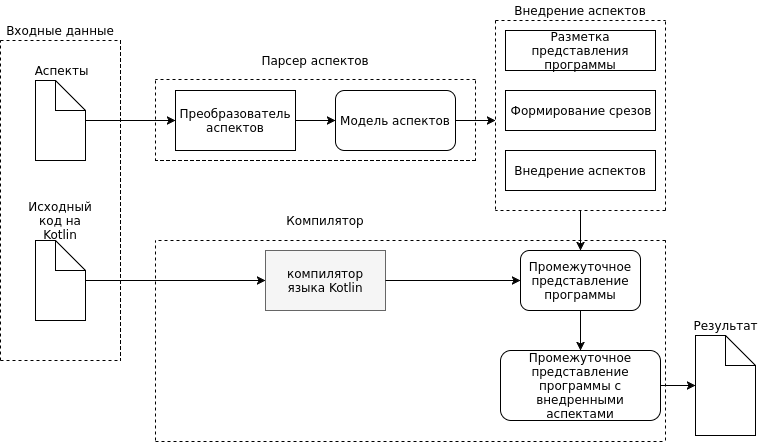
\includegraphics[width=\textwidth]{fig/program_architecture}
\caption{Архитектура программной системы}%
\label{fig:program_architecture}
\end{figure}

Как видно из рисунка~\ref{fig:program_architecture}, система состоит из
следующих частей:
\begin{enumerate}
	\item Первой частью системы являются преобразователи, отвечающие за
		 импортирование исходного кода и описания аспектов и приведения их к
		 виду промежуточного представления.
		 Для создания преобразователя аспектов, необходимо сформировать
		 грамматику описания аспектов.
		 Создание промежуточного представления программы может быть переложено
		 на компилятор языка Kotlin.
	\item Второй частью системы является часть, отвечающая за внедрение аспектов
		в промежуточное представление программы.
		Данная часть состоит из нескольких компонентов: части, отвечающей за
		разметку промежуточного представления, части, отвечающей за формирование
		срезов и части, реализующей внедрение аспектов.
	\item Последней частью системы является часть, отвечающая за компиляцию
		модифицированного промежуточного представления программы в байт-код.
		Данную часть также нет необходимости реализовывать полностью самому, так
		как можно воспользоваться готовыми системами сборки, передав в них
		не исходные коды программы, а модифицированное промежуточное
		представление.
\end{enumerate}

Таким образом, основное внимание стоит уделить модулям, отвечающим за построение
модели аспектов и внедрению аспектов в промежуточное представление программы.
%%%%%%%%%%%%%%%%%%%%%%%%%%%%%%%%%%%%%%%%%%%%%%%%%%%%%%%%%%%%%%%%%%%%%%%%%%%%%%%%
\section{Разработка синтаксиса аспектов}
\label{sec:aspect_syntax_design}
%%%%%%%%%%%%%%%%%%%%%%%%%%%%%%%%%%%%%%%%%%%%%%%%%%%%%%%%%%%%%%%%%%%%%%%%%%%%%%%%
По результатам анализа существующих АОП-расширений можно выделить два основных
способа описания аспектов: создание классов, каждый из которых позволяет
производить вставку кода советов или же использование дополнительного синтаксиса
описания аспектов.
Для разрабатываемого прототипа был выбран второй способ, а именно, создание
отдельного синтаксиса описания аспектов, схожего с описанием классов в языке
Kotlin.

За основу разрабатываемого синтаксиса было решено взять язык описания аспектов,
используемый в фреймворке AspectJ.
Данный выбор был сделан, во-первых, из-за большой популярности данного
АОП-расширения и, во-вторых, из-за удобства и гибкости данного способа описания
аспектов.
%%%%%%%%%%%%%%%%%%%%%%%%%%%%%%%%%%%%%%%%%%%%%%%%%%%%%%%%%%%%%%%%%%%%%%%%%%%%%%%%
\subsection{Синтаксис описания аспекта}
\label{sub:custom_aspect_syntax}
%%%%%%%%%%%%%%%%%%%%%%%%%%%%%%%%%%%%%%%%%%%%%%%%%%%%%%%%%%%%%%%%%%%%%%%%%%%%%%%%
Как и в AspectJ, сквозная функциональность инкапсулируется в сущности,
называемой \textit{аспект}.
Каждый аспект имеет свой уникальный идентификатор и может содержать как описание
советов и срезов, так и переменные и функции, предназначенные для внутреннего
использование.
Описание аспекта, в целом, похоже на описание класса в языке Kotlin: оно
начинается с ключевого слова \textit{aspect}, после чего следует идентификатор
аспекта и, затем, тело аспекта, заключенное в фигурные скобки.
Пример описания аспекта с идентификатором \textit{FooAspect} приведен в листинге
~\ref{lst:custom_aspect_example}.
  \begin{lstlisting}[language=Java, label={lst:custom_aspect_example}, 
  caption={Пример описания аспекта в разрабатываемом прототипе}]
aspect FooAspect  {
  ... Тело аспекта
}
  \end{lstlisting}
%%%%%%%%%%%%%%%%%%%%%%%%%%%%%%%%%%%%%%%%%%%%%%%%%%%%%%%%%%%%%%%%%%%%%%%%%%%%%%%%
\subsection{Синтаксис описания срезов}
\label{sub:custom_pointcut_syntax}
%%%%%%%%%%%%%%%%%%%%%%%%%%%%%%%%%%%%%%%%%%%%%%%%%%%%%%%%%%%%%%%%%%%%%%%%%%%%%%%%
За основу синтаксиса описания срезов был также взят фреймворк AspectJ.
Описание среза начинается с ключевого слова \textit{pointcut}, после чего
следует идентификатор среза, уникальный в рамках данного аспекта, перечень
аргументов и, непосредственно, описание среза.
При описании среза могут использоваться следующие конструкции:
\begin{itemize}
	\item \textit{call(паттерн\_метода)} --- вызов метода, указанного в
		  описании.
	\item \textit{execution(паттерн\_метода)} --- выполнение метода,
		  указанного в описании.
\end{itemize}

Описание метода также состоит из нескольких частей, описанных ниже в порядке их
следования:
\begin{enumerate}
	\item \textit{аннотации метода} --- необязательный параметр, содержащий
		  список аннотаций.
		  Можно задавать как обязательное наличие, так и отсутствие определенной
		  аннотации при помощи символа \quotes{!}.
	\item \textit{модификаторы метода} --- необязательный параметр, содержащий
		  описание модификаторов метода.
		  Может принимать следующие значения: public, private, protected,
		  internal, synchronized, final.
		  Можно задавать как обязательное наличие, так и отсутствие какого-либо
		  модификатора при помощи символа \quotes{!}.
	\item \textit{extension модификатор} --- необязательный параметр, задающий,
		  является ли функция \quotes{расширением} или нет.
	\item ключевое слово \quotes{fun}.
	\item \textit{название пакета} --- необязательный параметр, задающий имя
		  пакета и класса, в котором объявлена функция.
		  Возможен пропуск одного или нескольких символов, при помощи символа
		  \quotes{*}.
	\item \textit{имя функции} --- обязательный параметр, задающий имя функции.
		  Возможен пропуск одного или нескольких символов, при помощи символа
		  \quotes{*}.
	\item \textit{список типов параметров функции} --- необязательны параметр,
		  задающий список типов аргументов, которые имеет функция, в
		  соответствующем порядке.
		  В качестве типов, могут использоваться как стандартные типы языка
		  Kotlin, как, например, Double, Int, Short и т.д., так и
		  пользовательские типы данных.
		  Опционально можно указывать соответствие параметров функции на
		  \quotes{NotNull} и \quotes{Nullable} при помощи модификаторов
		  \quotes{!!} и \quotes{?} соответственно.
		  Если количество и типы аргументов функции не имеет значения, то это
		  можно указать, используя символ \quotes{..}.
		  Список параметров оборачивается в круглые скобки.
	\item \textit{тип возвращаемого значения} --- необязательный параметр,
		  показывающий тип значения, возвращаемого функцией.
		  В качестве типа, могут использоваться как стандартные типы языка
		  Kotlin, как, например, Double, Int, Short и т.д., так и
		  пользовательские типы данных.
		  Также как и при указании параметров функции, типу возвращаемого
		  значения можно задавать соответствие на \quotes{NotNull} и
		  \quotes{Nullable} при помощи модификаторов \quotes{!!} и \quotes{?}.
		  При указании типа возвращаемого значения, оно отделяется от списка
		  аргументов символом \quotes{:}, по аналогии с описанием функций на
		  языке Kotlin.
\end{enumerate}

Данные конструкции могут группироваться между собой при помощи следующих
логических операций \textit{конъюнкции} (\&\&),  \textit{дизъюнкции} (||)  и
\textit{инверсии} (!).
При описании срезов могут использоваться не только 
%%%%%%%%%%%%%%%%%%%%%%%%%%%%%%%%%%%%%%%%%%%%%%%%%%%%%%%%%%%%%%%%%%%%%%%%%%%%%%%%
\subsection{Синтаксис описания советов}
\label{sub:custom_advice_syntax}
%%%%%%%%%%%%%%%%%%%%%%%%%%%%%%%%%%%%%%%%%%%%%%%%%%%%%%%%%%%%%%%%%%%%%%%%%%%%%%%%
Описание советов также во многом схоже с описанием, используемым в AspectJ.
Оно начинается с ключевого слова, описывающего способ внедрения
кода совета относительно точки объединения, а именно:
\begin{itemize}
	\item \textit{before} --- вставка кода совета до точки объединения;
	\item \textit{after} --- вставка кода совета после точки объединения;
	\item \textit{around} --- вставка кода совета до и после точки объединения;
\end{itemize}
После этого могут следовать аргументы функций, к которым будет производиться
обращение внутри кода совета.

Следующей частью совета является описание среза, аналогичное представленному в
разделе~\ref{sub:custom_pointcut_syntax}, после которого следует код совета,
представляющий из себя программный код на языке Kotlin.
%%%%%%%%%%%%%%%%%%%%%%%%%%%%%%%%%%%%%%%%%%%%%%%%%%%%%%%%%%%%%%%%%%%%%%%%%%%%%%%%
\section{Внедрение аспектов}
\label{sub:custom_aspect_weaving}
%%%%%%%%%%%%%%%%%%%%%%%%%%%%%%%%%%%%%%%%%%%%%%%%%%%%%%%%%%%%%%%%%%%%%%%%%%%%%%%%
Первая часть данного раздел посвящена описанию промежуточного представления,
создаваемому в процессе компиляции программ на Kotlin.
Во второй части будет приведено описание способа применения аспектов к PSI.
%%%%%%%%%%%%%%%%%%%%%%%%%%%%%%%%%%%%%%%%%%%%%%%%%%%%%%%%%%%%%%%%%%%%%%%%%%%%%%%%
\subsection{Описание PSI}
\label{sub:psi_description}
%%%%%%%%%%%%%%%%%%%%%%%%%%%%%%%%%%%%%%%%%%%%%%%%%%%%%%%%%%%%%%%%%%%%%%%%%%%%%%%%
\nomenclature{PSI}{Program Structure Interface}
Язык Kotlin имеет ряд оригинальных языковых конструкций (extension функции,
специфичные лямбда-функции и т.п.), при этом основной целевой платформой
компиляции для языка Kotlin является JVM.
Как результат --- все специальные конструкции Kotlin преобразуются в стандартный
байт-код, который имеет одинаковую структуру и для Java, и для Kotlin-программ.
Не смотря на то, что в версии языка Kotlin 1.1.1 часть специфичных для языка
Kotlin конструкций можно выбелить при помощи Reflection, некоторые конструкции,
как например inline функции невозможно.
%% Предложение выше неплохо бы уточнить
Из-за этого поиск некоторых структур языка Kotlin в байт-коде становится
затруднительным и, как следствие, динамическое внедрение кода советов при
загрузке файлов в JVM становится практически невозможным.
По той же причине статическое внедрение советов в байт-код программы также
является очень сложной задачей.

Таким образом, в качестве способа внедрения аспектов было выбрано внедрение аспектов в исходный код программы или в модель программы во время компиляции. 

Разработчики языка Kotlin предусмотрели специальную структуру данных для работы
с программным кодом --- Program Structure Interface (PSI), более.
В нашем проекте мы используем PSI для внедрения объектов на этапе компиляции
проекта.

\textit{PSI} --- промежуточное представление программного кода, используемого
разработчиками языка Kotlin при компиляции.
PSI представляет из себя набор виртуальных файлов~\cite{psi_file},
соответствующих реальным файлам с исходными кодами программы.
Каждый виртуальный файл, помимо информации о соответствующем реальном файле,
содержит дерево разбора содержимого файла, представленного в виде иерархии
объектов, типа \textit{PsiElement}~\cite{psi_element}.
Виртуальный файл также является наследником интерфейса PsiElement.
%%%%%%%%%%%%%%%%%%%%%%%%%%%%%%%%%%%%%%%%%%%%%%%%%%%%%%%%%%%%%%%%%%%%%%%%%%%%%%%%
\subsubsection{Интерфейс PsiElement}
\label{ssub:psi_element_description}
%%%%%%%%%%%%%%%%%%%%%%%%%%%%%%%%%%%%%%%%%%%%%%%%%%%%%%%%%%%%%%%%%%%%%%%%%%%%%%%%
Интерфейс PsiElement является базовым интерфейсом, от которого унаследованы все
элементы, являющиеся узлами PSI.
Он содержит множество функций для манипуляций с PSI, однако, при проектировании
АОП-расширения, нас, в первую очередь, интересуют следующее:
\begin{itemize}
	\item \textit{Project getProject()} --- метод, возвращающий проект, к
		которому относится данный элемент.
	\item \textit{PsiElement[] getChildren()} --- метод, возвращающий список
		дочерних элементов данного элемента.
	\item \textit{PsiElement getParent()} --- метод, возвращающий родительский
		элемент.
	\item \textit{String getText()} --- метод, возвращающий текстовое
		представление элемента.
	\item \textit{PsiElement copy()} --- метод, возвращающий копию данного
		элемента.
	\item \textit{PsiElement add(@NotNull PsiElement element) throws
		IncorrectOperationException} --- метод, позволяющий добавлять потомка
		\textit{element} к данному элементу.
		Данный метод возвращает фактически добавленный элемент или его копию.
	\item \textit{PsiElement addBefore(@NotNull PsiElement element, @Nullable
		PsiElement anchor) throws IncorrectOperationException} --- метод,
		позволяющий добавлять элемент \textit{element} перед элементом
		\textit{anchor}.
		Данный метод возвращает фактически добавленный элемент или его копию.
	\item \textit{PsiElement addAfter(@NotNull PsiElement element, @Nullable
		PsiElement anchor) throws IncorrectOperationException} --- метод,
		позволяющий добавлять элемент \textit{element} после элемента
		\textit{anchor}.
		Данный метод возвращает фактически добавленный элемент или его копию.
	\item \textit{void checkAdd(@NotNull PsiElement element) throws
		IncorrectOperationException} --- метод, проверяющий возможность
		добавления потомка \textit{element} к текущему элементу.
		В случае, если операция невозможна по каким-либо причинам, выбрасывается
		исключение \textit{IncorrectOperationException}.
	\item \textit{PsiElement replace(@NotNull PsiElement newElement) throws
		IncorrectOperationException} --- метод, позволяющий заменять текущий
		элемент, элементом \textit{newElement}.
		Данный метод возвращает элемент, который был добавлен в дерево.
	\item \textit{<T> T getCopyableUserData(Key<T> key)} --- метод, возвращающий
		пользовательские данные, находящиеся в структуре \textit{myUserData}
		с ключем \textit{key}.
	\item \textit{<T> void putCopyableUserData(Key<T> key, @Nullable T value)}
		--- метод, позволяющий сохранить пользовательские данные
		\textit{value}, в структуре \textit{myUserData} под ключем \textit{key}.
\end{itemize}
%%%%%%%%%%%%%%%%%%%%%%%%%%%%%%%%%%%%%%%%%%%%%%%%%%%%%%%%%%%%%%%%%%%%%%%%%%%%%%%%
\subsubsection{Класс KtCallExpression}
\label{ssub:kt_call_expression_description}
%%%%%%%%%%%%%%%%%%%%%%%%%%%%%%%%%%%%%%%%%%%%%%%%%%%%%%%%%%%%%%%%%%%%%%%%%%%%%%%%
Класс \textit{KtCallExpression} представляет узел, соответствующий вызову
функции.
В разрабатываемом расширении предполагается использовать следующие методы
данного класса:
\begin{itemize}
	\item \textit{getResolvedCall(context: BindingContext): ResolvedCall
		<CallableDescriptor>?} --- метод, позволяющий получать дескриптор
		вызываемой функции.
\end{itemize}
%%%%%%%%%%%%%%%%%%%%%%%%%%%%%%%%%%%%%%%%%%%%%%%%%%%%%%%%%%%%%%%%%%%%%%%%%%%%%%%%
\subsubsection{Класс KtNamedFunction}
\label{ssub:kt_named_function_description}
%%%%%%%%%%%%%%%%%%%%%%%%%%%%%%%%%%%%%%%%%%%%%%%%%%%%%%%%%%%%%%%%%%%%%%%%%%%%%%%%
Класс \textit{KtNamedFunction} представляет узел, соответствующий объявлению
именованной функции.
В разрабатываемом расширении предполагается использовать следующие методы
данного класса:
\begin{itemize}
	\item \textit{getResolvedCall(context: BindingContext): ResolvedCall
		<CallableDescriptor>?} --- метод, позволяющий получать дескриптор
		вызываемой функции.
	\item \textit{getValueParameters(): MutableList<KtParameter>} --- метод,
		позволяющий получить список аргументов, принимаемых функцией в виде
		списка элементов типа \textit{KtParameter}.
	\item \textit{hasDeclaredReturnType(): Boolean} --- метод, позволяющий
		узнать, возвращает ли функция какое-либо значение или нет.
	\item \textit{getTypeReference(): KtTypeReference?} --- метод, позволяющий
		получить тип возвращаемого функцией значения.
	\item \textit{isExtensionDeclaration(): Boolean} --- метод, позволяющий
		проверить является ли данная функция extension или нет.
	\item \textit{isPrivate(): Boolean} --- метод, позволяющий проверить,
		является ли данная функция приватной.
	\item \textit{isProtected(): Boolean} --- метод, позволяющий проверить,
		является ли данная функция protected.
	\item \textit{getModifierList(): KtModifierList?} --- метод, позволяющий
		получить список модификаторов функции.
		Данный метод возвращает экземпляр класса \textit{KtModifierList}, содержащий
		в списке узлов модификаторы функции.
\end{itemize}
%%%%%%%%%%%%%%%%%%%%%%%%%%%%%%%%%%%%%%%%%%%%%%%%%%%%%%%%%%%%%%%%%%%%%%%%%%%%%%%%
\subsubsection{CallableDescriptor}
\label{ssub:callable_descriptor_description}
%%%%%%%%%%%%%%%%%%%%%%%%%%%%%%%%%%%%%%%%%%%%%%%%%%%%%%%%%%%%%%%%%%%%%%%%%%%%%%%%
Класс \textit{CallableDescriptor} представляет узел, соответствующий
дескриптору вызываемой функции.
В разрабатываемом расширении предполагается использовать следующие методы
данного класса:
\begin{itemize}
	\item \textit{getName(): Name} --- метод, возвращающий имя функции в виде
		экземпляра типа \textit{Name}.
	\item \textit{getExtensionReceiverParameter(): ReceiverParameterDescriptor}
		--- метод, позволяющий получить имя класса и пакета, к которому принадлежит
		 extension функция.
	\item \textit{getContainingDeclaration(): DeclarationDescriptor} --- метод,
		позволяющий получить имя класса и пакета, к которому принадлежит не
		extension функция.
	\item \textit{getValueParameters(): MutableList<ValueParameterDescriptorImpl>}
		--- метод, позволяющий получить список аргументов, принимаемых функцией в виде списка элементов типа \textit{ValueParameterDescriptorImpl}.
	\item \textit{getReturnType(): KotlinType?} --- метод, позволяющий получить
		тип возвращаемого функцией значения.
	\item \textit{isExtension(): Boolean} --- метод, позволяющий проверить
		является ли данная функция extension или нет.
	\item \textit{isInline(): Boolean} --- метод, позволяющий проверить
		является ли данная функция inline или нет.
	\item \textit{getVisibility(): Visibility} --- метод, позволяющий получить
		класс, содержащий в себе видимость функции (является ли функция \textit{public}, или \textit{private}, или \textit{protected}).
\end{itemize}
%%%%%%%%%%%%%%%%%%%%%%%%%%%%%%%%%%%%%%%%%%%%%%%%%%%%%%%%%%%%%%%%%%%%%%%%%%%%%%%%
\subsection{Формирование срезов}
\label{ssec:pointcut_creation_description}
%%%%%%%%%%%%%%%%%%%%%%%%%%%%%%%%%%%%%%%%%%%%%%%%%%%%%%%%%%%%%%%%%%%%%%%%%%%%%%%%
Формирование набора точек внедрения также происходит в несколько шагов.
На первом шаге, каждый узел PSI проверяется на соответствие каждому из отдельно
описанных внутри совета срезов.
В случае, если узел подходит данному срезу, то в структуру userMap добавляется
идентификатор этого среза.
На втором шаге, после того, как дерево было размечено идентификаторами срезов, 
для каждого совета проверяется, можно ли его применить к данному узлу дерева.
Если можно, то происходит внедрение кода совета в соответствующую позицию
относительно точки внедрения.
%%%%%%%%%%%%%%%%%%%%%%%%%%%%%%%%%%%%%%%%%%%%%%%%%%%%%%%%%%%%%%%%%%%%%%%%%%%%%%%%
\subsection{Применение кода советов}
\label{ssec:advice_applying_description}
%%%%%%%%%%%%%%%%%%%%%%%%%%%%%%%%%%%%%%%%%%%%%%%%%%%%%%%%%%%%%%%%%%%%%%%%%%%%%%%%
Внедрение аспектов происходит в несколько этапов, схематически изображенных на
рисунке~\ref{fig:aspect_weaving}.
\begin{figure*}[!t]
\centering
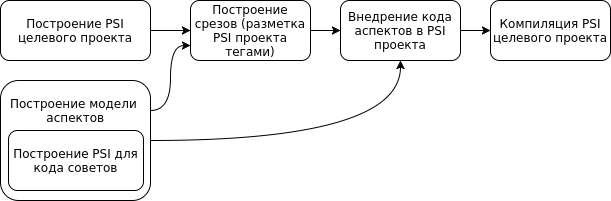
\includegraphics[width=1\textwidth]{fig/aspect_weaving}
\caption{Процесс внедрения аспектов в программный код при компиляции}
\label{fig:aspect_weaving}
\end{figure*}

Первым этапом является построение PSI, подробно описанного в разделе~\ref{sub:psi_description}.
Каждый элемент дерева разбора содержит в себе текст соответствующего элемента,
ссылки на потомков и различную сопровождающую информацию.
Одним из таких полей является <<userMap>> типа \textit{KeyFMap} --- структура в,
которую могут быть записаны различные пользовательские данные.

Вторым этапом является чтение файлов с описаниями аспектов и формирование
модели аспектов, состоящих из срезов и советов.
Каждый экземпляр совета и среза содержит:
\begin{itemize}
	\item уникальный идентификатор, используемый для разметки PSI;
	\item дерево разбора логического выражения, используемое при анализе
		  принадлежности точки срезу.
\end{itemize}
Также экземпляр совета содержит в себе код совета, приведенный к виду
промежуточного представления для более удобной модификации PSI.
Дерево разбора в качестве нетерминальных узлов содержит в себе логические
операции <<и>>, <<или>>, <<не>>.
Терминальными же узлами выступают или сигнатуры, используемые для описания
срезов, или же идентификаторы других срезов.

При внедрении в PSI код советов оборачивается в лямбда функцию \textit{run}, что
позволяет разрешать сложные случаи, например, при последовательном вызове
нескольких функций без создания большого числа дополнительных 
промежуточных переменных.
Для наглядности, рассмотрим участок кода в листинге~\ref{target_ex}.
\begin{lstlisting}[label=target_ex,
    caption={Пример целевой точки внедрения}]
...
val res = A.foo().bar().baz()
...
\end{lstlisting}
При необходимости применить совет непосредственно после вызова функции 
\textit{bar()} целевая функция оборачивается в метод \textit{run}, значение, 
возвращаемое функцией присваивается некоторой промежуточной переменной, после 
чего вставляется код совета и затем из блока возвращается переменная, 
содержащая результат, возвращенный функцией \textit{bar}, к которой был применен
совет.
Результат преобразования представлен в листинге~\ref{apply_advice_ex}.
\begin{lstlisting}[label=apply_advice_ex,
    caption={Пример внедрения кода с использованием функции run}]
...
val res = A.foo().run{
        val buf = bar()
        //advice code
        buf
    }.baz()
...
\end{lstlisting}

Данный подход решает проблему разнесения вложенного вызова методов, при котором 
пришлось бы заводить множество временных переменных, а также контролировать 
возвращаемые результаты методов.
К недостаткам данного подхода можно отнести то, что при изменении аспекта,
требуется полная перекомпиляция проекта.
Однако, при таком подходе, нет необходимости производить дополнительные действия
при запуске для корректной работы полученного jar файла.
%%%%%%%%%%%%%%%%%%%%%%%%%%%%%%%%%%%%%%%%%%%%%%%%%%%%%%%%%%%%%%%%%%%%%%%%%%%%%%%%
\section{Выводы}
\label{sec:design_conclusion}
%%%%%%%%%%%%%%%%%%%%%%%%%%%%%%%%%%%%%%%%%%%%%%%%%%%%%%%%%%%%%%%%%%%%%%%%%%%%%%%%
%%%%%%%%%%%%%%%%%%%%%%%%%%%%%%%%%%%%%%%%%%%%%%%%%%%%%%%%%%%%%%%%%%%%%%%%%%%%%%%%
